\section{Технический проект}
\subsection{Общая характеристика организации решения задачи}

Необходимо спроектировать и разработать игру, которая должна соответствовать всем предъявленным к ней требованиям.

Компьютерная игра — это форма развлечения, предназначенная для запуска и игры на компьютере. Она включает в себя визуальные, звуковые и интерактивные элементы, предоставляя пользователю виртуальное окружение, где тот может взаимодействовать с созданным миром, управлять персонажами и решать различные задачи. Компьютерные игры могут быть разнообразными и включать в себя различные жанры, такие как стратегии, шутеры, головоломки, ролевые игры, платформеры и другие.

\subsection{Обоснование выбора технологии проектирования}

На сегодняшний день информационный рынок, поставляющий программные решения в выбранной сфере, предлагает множество продуктов, позволяющих достигнуть поставленной цели – разработки игры.

\subsubsection{Описание используемых технологий и языков программирования}

В процессе разработки игры используются язык программирования и программные средства, которые применяются для круга задач, при решении которых они необходимы.

\subsubsection{Язык программирования Python}

Питон (Python) - высокоуровневый язык программирования общего назначения с динамической строгой типизацией и автоматическим управлением памятью, ориентированный на повышение производительности разработчика, читаемости кода и его качества, а также на обеспечение переносимости написанных на нём программ.

\paragraph{Достоинства языка Python}

Вот некоторые из основных достоинств Python:

\begin{enumerate}
	\item Простота и читаемость кода:
	
	Python ставит акцент на читаемости кода, что делает его пригодным для быстрого и легкого написания программ. Ясный и понятный синтаксис помогает новичкам и специалистам одинаково.
	\item Интерпретируемость:
	
	Интерпретируемость Python обеспечивает быструю разработку и тестирование кода. Без необходимости компиляции, изменения могут быть внесены и протестированы непосредственно.
	\item Обширная стандартная библиотека:
	
	Python поставляется с обширной стандартной библиотекой, предоставляя разработчикам множество инструментов и модулей для решения разнообразных задач, таких как работа с файлами, сетевое программирование, обработка данных, создание игр и многое другое.
	\item Объектно-ориентированное программирование:
	
	Python поддерживает объектно-ориентированное программирование (ООП), что позволяет создавать модульный и структурированный код, упрощая его повторное использование и сопровождение.
	\item Динамическая типизация:
	
	Динамическая типизация Python позволяет гибко использовать переменные, не требуя их явного объявления типа. Это упрощает написание и изменение кода.
	\item Поддержка сторонних библиотек и фреймворков:
	
	Существует огромное количество сторонних библиотек и фреймворков для Python, таких как Django для веб-разработки, NumPy и Pandas для анализа данных, TensorFlow для машинного обучения, Pygame для игр, что делает его мощным инструментом в различных областях.
	\item Переносимость:
	
	Python является кроссплатформенным, что означает, что программы, написанные на Python, могут быть запущены на различных операционных системах без изменений кода.
\end{enumerate}

\paragraph{Недостатки языка Python}

Хотя Python является мощным и популярным языком программирования, у него также есть некоторые недостатки, которые могут влиять на выбор его использования в конкретных сценариях. Вот несколько из них:

\begin{enumerate}
	\item Производительность:
	
	Python обычно менее эффективен в выполнении определенных задач по сравнению с компилируемыми языками, такими как C++ или Java. Это особенно заметно в вычислительно интенсивных приложениях.
	\item Поддержка мобильной разработки:
	
	Python не является основным языком для мобильной разработки, хотя существуют некоторые фреймворки, такие как Kivy или BeeWare, которые позволяют создавать мобильные приложения на Python. Однако в данном контексте часто предпочитаются другие языки, такие как Java (Android) или Swift (iOS).
	\item Глобальная блокировка интерпретатора (GIL):
	
	GIL в Python представляет собой ограничение, которое позволяет только одному потоку исполнения выполняться в определенный момент времени. Это может стать проблемой в многопроцессорных системах, где несколько ядер могут оставаться неиспользуемыми.
	\item Объем памяти:
	
	Python может потреблять больше памяти по сравнению с некоторыми языками программирования из-за своей динамической природы.
	\item Отсутствие некоторых особенностей в сравнении с компилируемыми языками:
	
	Python может не подходить для разработки низкоуровневых систем или приложений, требующих максимальной производительности и полного контроля над ресурсами
\end{enumerate}

\subsection{Диаграмма компонентов и схема обмена данными между файлами компонента}

Диаграмма компонентов описывает особенности физического представления разрабатываемой игры. Она позволяет определить архитектуру игры, установив зависимости между программными компонентами, в роли которых может выступать как исходный, так и исполняемый код. Основными графическими элементами диаграммы компонентов являются компоненты, интерфейсы, а также зависимости между ними. На рисунке \ref{comp:image} изображена диаграмма компонентов для проектируемой игры. Она включает в себя игровое окно, в котором отображены счет и игровые объекты. Они делятся на собираемые предметы, препятствия, платформы, объект выхода и объект игрока.

\begin{figure}[ht]
\center{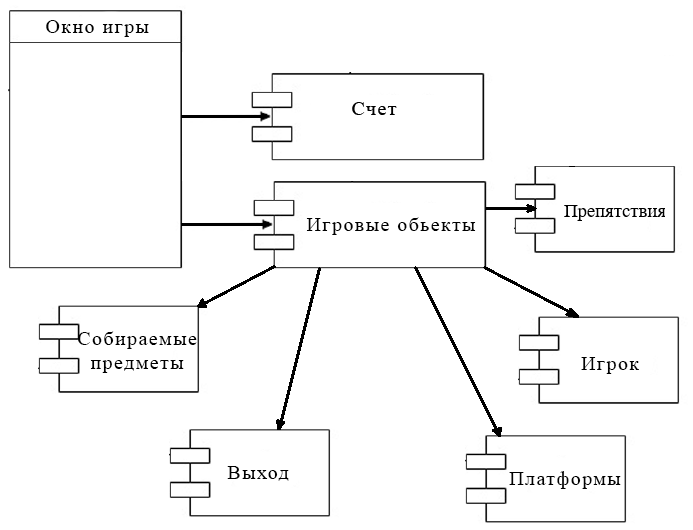
\includegraphics[width=1\linewidth]{comp}}
\caption{Диаграмма компонентов}
\label{comp:image}
\end{figure}

Любой компонент должен быть вызван в сценарии игры. Игра передает данные компоненту в момент вызова последнего.

На рисунке \ref{data:image} представлена схема обмена данными между сценариями игры при взаимодействии компонентов.

\begin{figure}[ht]
\center{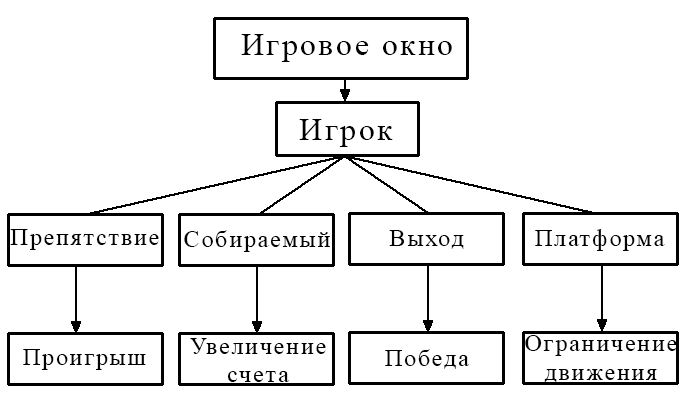
\includegraphics[width=1\linewidth]{data}}
\caption{Диаграмма компонентов}
\label{data:image}
\end{figure}

При взаимодействии с компонентом в сценарии игры происходит распознавание взаимодействующих объектов.

При взаимодействии игрока с разными объектами происходят разные действия. Например при соприкосновении с платформой сбоку игрок не может идти дальше, если платформа находится сверху игрок не может прыгнуть выше и ударяется об нее, если она снижу игрок перестает падать и останавливается на платформе. При соприкосновении игрока с собираемыми предметами, они удаляются с экрана и увеличивают счет. При соприкосновении игрока с препятствие игрок проигрывает. При соприкосновении игрока с выходом, если собраны все предметы, уровень завершается.

Работа компонента заканчивается в момент завершения работы сценария игры или удаления компонента с экрана.

\subsection{Основные сущности игры}

Проанализировав требования, можно выделить две основных сущности:
\begin{itemize}
\item "<Игровой объект">;
\item "<Анимация">.
\end{itemize}

В состав сущности "<Игровой объект"> можно включить атрибуты, представленные в таблице \ref{news:table}.

\begin{xltabular}{\textwidth}{|l|l|p{1.7cm}|X|}
	\caption{Атрибуты сущности "<Игровой объект">\label{news:table}}\\ \hline
	\centrow Поле & \centrow Тип & \centrow Обяза\-тельное & \centrow Описание \\ \hline
	\thead{1} & \thead{2} & \centrow 3 & \centrow 4 \\ \hline
	\endfirsthead
	\thead{1} & \thead{2} & \centrow 3 & \centrow 4 \\ \hline
	\finishhead
	\ id & int & true & Уникальный идентификатор \\ \hline 
	tag & str & true & тег объекта \\ \hline 
	animations & Animation & false & Анимации объекта \\ \hline 
	currentAnim & str & false & Ключ текущей анимации
\end{xltabular}

В состав сущности "<Анимация"> можно включить атрибуты, представленные в таблице \ref{news:table}.

\begin{xltabular}{\textwidth}{|l|l|p{1.7cm}|X|}
	\caption{Атрибуты сущности "<Анимация">\label{news:table}}\\ \hline
	\centrow Поле & \centrow Тип & \centrow Обяза\-тельное & \centrow Описание \\ \hline
	\thead{1} & \thead{2} & \centrow 3 & \centrow 4 \\ \hline
	\endfirsthead
	\thead{1} & \thead{2} & \centrow 3 & \centrow 4 \\ \hline
	\finishhead
	\ frame & int & true & Индекс кадра \\ \hline 
	time & int & true & Скорость анимации \\ \hline 
	name & str & true & Название анимации \\ \hline 
	anim & list[PhotoImage] & true & Список кадров \\ \hline
	n & int & true & Количество кадров \\ \hline
	filename & str & true & Имя файла
\end{xltabular}